\documentclass[11pt,a4paper]{article}
\usepackage[margin=0.85in]{geometry}
\usepackage{graphicx,booktabs,amsmath,amssymb,xcolor,float}
\usepackage[colorlinks=true,linkcolor=blue,urlcolor=blue]{hyperref}
\usepackage{caption}
\usepackage{subcaption}
\usepackage{enumitem}
\setlist{itemsep=1pt,topsep=3pt}
% long \texttt{} spans cannot hyphenate; allow extra stretch so lines
% fit instead of running into the margin
\setlength{\emergencystretch}{3em}
\graphicspath{{../out/figs/}}
\newcommand{\NtrainSplit}{8{,}442}
\newcommand{\NvalSplit}{2{,}111}
\newcommand{\Nfit}{3{,}000}
\newcommand{\Ntest}{5{,}019}
\newcommand{\valMIoU}{0.7305}
\newcommand{\valIoUbg}{0.8393}
\newcommand{\valIoUob}{0.6218}
\newcommand{\valBF}{0.4660}
\newcommand{\valQ}{0.6512}
\newcommand{\valCES}{0.5896}
\newcommand{\Nval}{2111}
\newcommand{\teMIoU}{0.6115}
\newcommand{\teIoUbg}{0.8326}
\newcommand{\teIoUob}{0.3904}
\newcommand{\teBF}{0.3737}
\newcommand{\teQ}{0.5402}
\newcommand{\teCES}{0.4891}
\newcommand{\Nte}{5019}
\newcommand{\capMIoU}{0.7351}
\newcommand{\capIoUbg}{0.8623}
\newcommand{\capIoUob}{0.6080}
\newcommand{\capBF}{0.4024}
\newcommand{\capQ}{0.6353}
\newcommand{\capCES}{0.5752}
\newcommand{\Ncap}{8}
\newcommand{\timePen}{0.0945}
\newcommand{\sizePen}{0.00015}
\newcommand{\cesMult}{0.9054}
\newcommand{\timePenPct}{9.4}
\newcommand{\phaseMean}{8.8}
\newcommand{\phasePfive}{4}
\newcommand{\phasePnine}{15}
\newcommand{\Tcpu}{23.62}
\newcommand{\Tpfifty}{23.42}
\newcommand{\Tpninenine}{31.91}
\newcommand{\Tmax}{64.85}
\newcommand{\Ntimed}{5{,}019}
\newcommand{\Sdisk}{6{,}238}
\newcommand{\SdiskMiB}{0.006}
\newcommand{\workRes}{128}
\newcommand{\gridG}{16}
\newcommand{\nRegions}{256}
\newcommand{\kmIters}{4}
\newcommand{\lamVal}{32}
\newcommand{\sigmaMult}{0.15}
\newcommand{\compactness}{10}


\title{\vspace{-1.6cm}\textbf{Cost-Efficient Segmentation under a Compute Budget}\\[2pt]
\large CSL7360: Computer Vision --- Assignment 2 (Track A: Classical)}
\author{Lakshya Jain \quad (B23CS1032)}
\date{November 2026}

\begin{document}
\maketitle
\vspace{-0.8cm}

\section{Objective and summary}
The task is to label every pixel of a $256\times256$ photo as \emph{main object} or
\emph{background}, using at most $50$\,ms of single-core CPU time per photo on average.
This is \textbf{Track A}: cluster the image into compact regions, learn a probability
that each region is object, and recover the labelling as the minimum cut of a graph over
those regions. The clustering, the region model, the max-flow solver and both metrics are
implemented from scratch with NumPy and OpenCV primitives only.

The pipeline runs in $\Tcpu$\,ms per photo with a $\Sdisk$-byte parameter file, reaching
$\mathrm{CES}=\teCES$ on DUTS-TE.

\begin{figure}[H]\centering
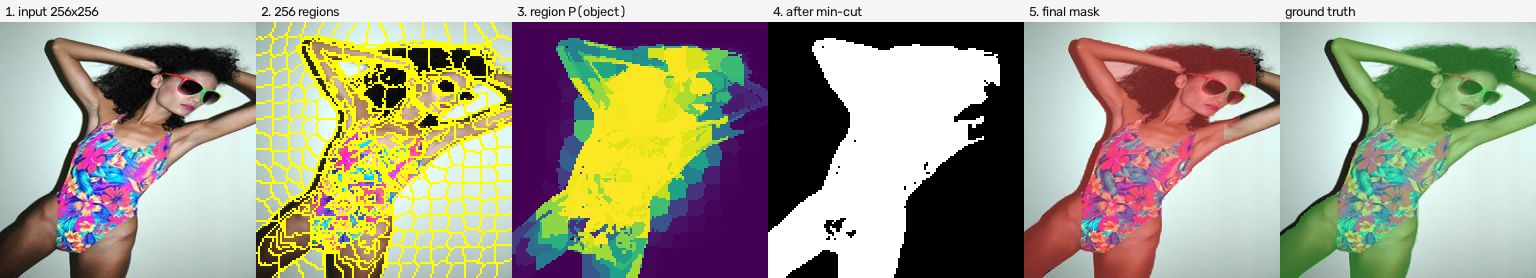
\includegraphics[width=\textwidth]{stages.png}
\caption{The pipeline on one validation image. The $256^2$ input is downscaled to
$\workRes^2$ and clustered into $\nRegions$ compact regions; a logistic regression over
17 region cues gives $P_p$; the min-cut of the region graph selects the object side;
the region labelling is expanded back to $256^2$. Red is the prediction, green the
ground truth.}
\end{figure}

\section{Data}
\textbf{Splits.} DUTS-TR (10{,}553 photos) is split \textbf{80/20} into
$\NtrainSplit$ training and $\NvalSplit$ validation photos with a fixed seed. All
design choices --- features, clustering resolution, $\lambda$ and $\sigma_d$ --- were
made on the validation split. The colour and position statistics and the logistic
regression were fitted on a $\Nfit$-photo subset of the training split, giving
$\approx$768k labelled regions for 170 parameters.
\textbf{DUTS-TE ($\Ntest$ photos) was never used for training, tuning, or any stopping
decision}; it was evaluated exactly once, at the end.

\textbf{Resizing.} Photos are resized to $256\times256$ with \texttt{cv2.INTER\_AREA}
and masks with \texttt{cv2.INTER\_NEAREST}; a mask pixel is object iff its value is
$\geq 128$. All metrics are computed on these $256\times256$ masks.

\textbf{Captured photos.} \Ncap{} photos taken around the campus/hostel, masked by hand
on the resized image. Together they cover all five listed conditions: indoor and
outdoor scenes, daylight and tube light, near and far objects, cluttered backgrounds,
and partial occlusion (Section~\ref{sec:captured}).

\section{Method}

\subsection{Clustering into regions}
Each pixel of the downscaled $\workRes\times\workRes$ image is described by
$(L,a,b,x,y)$, with the spatial coordinates scaled by $m/S$ where $m=\compactness$ is a
compactness constant and $S$ the grid spacing, which sets the trade-off between colour
and spatial distance. Centres are initialised on a regular $\gridG\times\gridG$ grid and
refined by $\kmIters$ rounds of Lloyd's algorithm.

Plain Lloyd's algorithm compares every pixel to every centre, costing $O(NK)$ per
sweep --- about $4.2$M distance evaluations here. Following SLIC, a pixel is compared
only against the grid centres nearest to it: the four nearest are determined by which
quadrant of its cell the pixel occupies, so assignment costs $O(4N)$, \emph{independent
of $K$}. The restriction also keeps clusters spatially compact and connected, which the
graph cut requires since it treats each cluster as a single node.

\subsection{Region descriptors}
For each region I compute 17 cues, all from vectorised \texttt{np.bincount} reductions:
\begin{itemize}
\item \textbf{Learned colour likelihood.} A $512$-bin Lab histogram of object and
background pixels is accumulated over the training subset; the per-region feature is the
mean of $\log P(c\mid\text{obj}) - \log P(c\mid\text{bg})$ over its pixels.
\item \textbf{Learned position prior.} A $16\times16$ map of $P(\text{object}\mid
\text{position})$ averaged over the training subset, again averaged over the region.
\item \textbf{Border contact} (fraction of the region's pixels on the image border),
area fraction, centroid offsets $|c_x-\tfrac12|,|c_y-\tfrac12|$.
\item \textbf{Contrast:} to the global mean colour, to the mean border colour, to
adjacent regions weighted by shared border length, and a spatially weighted
region-contrast term at two spatial scales.
\item \textbf{Diffused backgroundness.} Border regions are usually background, and that
evidence propagates to regions joined to them through colour-similar neighbours. Five
rounds of similarity-weighted averaging against the border seed approximate a random
walk on the region graph.
\item Mean $L,a,b$ and within-region colour spread (a flatness/texture proxy).
\end{itemize}

\subsection{Region probabilities}
$P_p$ comes from a logistic regression trained from scratch with Adam on a
\textbf{quadratic basis}: the 17 cues plus all pairwise products and squares, giving
170 weights. The problem stays convex, while the products let the model represent
interactions between cues that a linear surface over the 17 raw features cannot. Targets
are \emph{soft} --- the fraction of each region that is object --- so regions straddling
the boundary only partially pull the weights. Because of the basis expansion the
individual weights are not interpretable in isolation, so no single cue is reported as
dominant. Feature standardisation is folded back into $(w,b)$ after fitting, so
inference is a single dot product. Finally $P_p$ is clipped to $[0.001,0.999]$.

\subsection{Graph cut}
I build a graph with one node per region plus a source (object) and sink (background).
Following the specification, the source connects to region $p$ with capacity
$-\log(1-P_p)\,|p|$ and $p$ connects to the sink with capacity $-\log P_p\,|p|$, where
$|p|$ is the region's pixel count --- so the unary term is a sum over pixels,
commensurate with the pairwise term which is a sum over boundary pixel pairs. Cutting
the sink edge leaves $p$ on the source side, labelling it object and paying $-\log P_p$.

Two regions are adjacent if any of their pixels are 4-neighbours; they are joined in
both directions with weight $\lambda W_{pq}\,B_{pq}$, where $B_{pq}$ is the shared
border length and
\[
W_{pq}=\exp\!\left(-\frac{\lVert f(p)-f(q)\rVert^2}{2\sigma_d^2}\right),\qquad
\sigma_d^2 = \texttt{sigma\_mult}\cdot\overline{\lVert f(p)-f(q)\rVert^2} + 10^{-6},
\]
with $f$ the region mean colour and the average taken over that image's adjacent pairs.
So similar neighbours are expensive to separate. Tuning on validation gave
$\lambda=\lamVal$ and $\texttt{sigma\_mult}=\sigmaMult$.

Because the pairwise term is a Potts penalty it is submodular, so the binary labelling
that minimises this energy is recovered \emph{exactly} as a minimum s--t cut, rather
than approximately as with a greedy or thresholding scheme.

\textbf{Max-flow.} I implement \textbf{Dinic's algorithm} rather than Edmonds--Karp.
Both are augmenting-path methods, but Edmonds--Karp augments one shortest path per BFS
($O(VE^2)$), whereas Dinic's groups all shortest augmenting paths of a given length
into one phase: a BFS builds a level graph and a single DFS saturates a blocking flow
within it. The shortest $s$--$t$ distance strictly increases per phase, giving
$O(V^2E)$. Measured over 300 DUTS-TE photos these region graphs take a mean of
$\phaseMean$ phases (p5--p95: $\phasePfive$--$\phasePnine$), against hundreds of
individual augmentations for Edmonds--Karp. Capacities are scaled to integers so
termination is exact ---
with floats, repeated subtraction of near-zero residuals can stall the search.
The implementation was verified against a reference Edmonds--Karp on \textbf{2000
random graphs} (identical flow value on all of them), and the min-cut value was checked
to equal the max-flow value on every test.

\section{Staying inside the budget}
\label{sec:budget}
Clustering and max-flow over all 65{,}536 pixels in Python cannot fit in 50\,ms, so the
expensive stages run on the $\workRes^2$ downscale and on the $\nRegions$-node region
graph; only the final nearest-neighbour upsample touches $256^2$. Three measurements
drove the remaining design choices.

\textbf{Stage profile.} Max-flow accounts for a fifth of the runtime and clustering for
nearly half --- the opposite of what the algorithmic complexities suggest, because the
cut runs on a few hundred nodes while clustering runs on $\workRes^2$ pixels.

\begin{table}[H]\centering
\caption{Stage breakdown, 200 DUTS-TE photos. Per-stage instrumentation inflates the
total by ${\approx}15\%$ relative to the clean measurement of $\Tcpu$\,ms; the
proportions are what matter.}
\begin{tabular}{lrr}
\toprule
stage & ms & \% \\
\midrule
downscale + BGR$\to$Lab & 0.24 & 0.9 \\
grid-constrained K-Means & 12.90 & 46.8 \\
region descriptors + adjacency & 8.32 & 30.2 \\
logistic regression & 0.31 & 1.1 \\
graph build + Dinic min-cut & 5.61 & 20.4 \\
upsample to $256^2$ & 0.18 & 0.6 \\
\midrule
\textbf{total} & \textbf{27.56} & \textbf{100.0} \\
\bottomrule
\end{tabular}
\end{table}

\textbf{Two optimisations.} Restricting K-Means to the 4 nearest grid centres rather
than the full $3\times3$ neighbourhood, and dropping the constant $\lVert f\rVert^2$ term
so the distance reduces to a dot product, took clustering from $27.6$\,ms (9 candidates,
6 iterations) to $12.2$\,ms (4 candidates, 5 iterations), both measured at $112^2$.
Computing the region-contrast pairwise distances through the
$\lVert a\rVert^2-2a\!\cdot\!b+\lVert b\rVert^2$ expansion --- a small GEMM instead of an
$(M,M,3)$ broadcast --- recovered a further $4.8$\,ms. The freed budget was spent on the
contrast and diffusion cues.

\textbf{Oracle ceiling.} Labelling each region by its \emph{true} majority upper-bounds
any region-level method at a given granularity, separating clustering error from
region-model error.

\begin{table}[H]\centering
\caption{Region-oracle ceiling on 300 validation photos.}
\begin{tabular}{lccc}
\toprule
clustering & mIoU & BF1 & $Q$ \\
\midrule
$96^2$, 144 regions & 0.9447 & 0.7427 & 0.8841 \\
$128^2$, 256 regions & 0.9577 & 0.8047 & 0.9118 \\
$160^2$, 400 regions & 0.9662 & 0.8531 & 0.9323 \\
$192^2$, 576 regions & 0.9713 & 0.8874 & 0.9461 \\
\bottomrule
\end{tabular}
\end{table}

At $128^2$ the ceiling is $Q=0.912$ while the model achieves $\valQ$ on validation ---
so granularity is not the binding constraint --- the region model is. Moving to $192^2$
would raise the ceiling by $0.03$ while roughly doubling the runtime, so the resolution
was fixed at $\workRes^2$ and the remaining budget spent on region cues.

\section{Metrics}
Both metrics are implemented from scratch.

\textbf{mIoU.} One $2\times2$ confusion matrix is accumulated over the whole set, then
IoU is computed for background and for object and the two averaged.

\textbf{Boundary F1.} A boundary pixel is an object pixel with a background 4-neighbour,
with pixels outside the image counted as background (so a zero-padded shift is the right
comparison). The $5\times5$ tolerance test is a binary dilation, but \texttt{cv2.dilate}
is not permitted --- instead I convolve the binary boundary map with a $5\times5$ box of
ones using \texttt{cv2.filter2D}, which counts how many boundary pixels fall in each
window; testing count $>0$ is exactly dilation by a $5\times5$ structuring element. This
replaces the per-pixel Python loop the brief warns against and runs over all $\Ntest$
images in seconds. BF1 is computed per image and averaged; it is 1 if neither mask has
boundary pixels and 0 if only one does.

\section{Results}

\textbf{Measurement conditions.} Timing follows Section 2b exactly: all thread
environment variables set to \texttt{"1"} before importing NumPy/OpenCV, plus
\texttt{cv2.setNumThreads(1)} and \texttt{torch.set\_num\_threads(1)}; one warm-up run
discarded; then the $\Ntest$ DUTS-TE photos segmented one at a time, summing
\texttt{time.process\_time()}. The timed region starts with a $256\times256$ photo in
memory and ends with its $256\times256$ 0/1 mask, including the downscale and colour
conversion. \textbf{CPU: Intel Core i5-1340P} (laptop, single thread, no subprocesses).

\begin{table}[H]\centering
\caption{Main results. $Q=0.70\,\mathrm{mIoU}+0.30\,\mathrm{BF1}$;
$\mathrm{CES}=Q\left(1-0.20\frac{T_{\mathrm{CPU}}}{50\,\mathrm{ms}}
-0.10\min(1,\frac{S_{\mathrm{disk}}}{4\,\mathrm{MiB}})\right)$.}
\begin{tabular}{lrrrrr}
\toprule
set & $n$ & mIoU & BF1 & $Q$ & CES \\
\midrule
validation (DUTS-TR split) & \Nval & \valMIoU & \valBF & \valQ & \valCES \\
\textbf{DUTS-TE} & \Nte & \teMIoU & \teBF & \teQ & \textbf{\teCES} \\
captured photos & \Ncap & \capMIoU & \capBF & \capQ & \capCES \\
\bottomrule
\end{tabular}

\vspace{4pt}
{\footnotesize
$T_{\mathrm{CPU}} = \Tcpu$\,ms (median $\Tpfifty$, p99 $\Tpninenine$) over $\Ntimed$ photos
\quad $S_{\mathrm{disk}} = \Sdisk$ bytes $= \SdiskMiB$ MiB\\
time penalty $\timePen$ \quad size penalty $\sizePen$ \quad combined multiplier $\cesMult$}
\end{table}

At $\Tcpu$\,ms the time penalty removes $\timePenPct\%$ of $Q$ and the $\Sdisk$-byte
parameter file removes $0.015\%$. $Q$ therefore dominates CES, so optimisation effort
went to the region model rather than to further reducing runtime.

\subsection{Validation does not predict test here}
\label{sec:gap}
Validation $Q=\valQ$ but DUTS-TE $Q=\teQ$. This is not overfitting in the usual sense:
the model has 170 parameters fitted on ${\sim}768$k regions. The cause is a distribution
shift between the two halves of DUTS.

\begin{table}[H]\centering
\caption{Object size differs sharply between DUTS-TR and DUTS-TE.}
\begin{tabular}{lccc}
\toprule
& mean object fraction & median & photos with object $<5\%$ of frame \\
\midrule
DUTS-TR (validation split) & 0.271 & 0.256 & 4.7\% \\
DUTS-TE & 0.148 & 0.109 & 22.2\% \\
\bottomrule
\end{tabular}
\end{table}

DUTS-TE objects are roughly \textbf{half the size} and tiny objects are nearly
\textbf{five times more common}. The captured set is an independent check on this
reading: its objects average $21.2\%$ of the frame --- much closer to DUTS-TR than to
DUTS-TE --- and its score ($Q=\capQ$) lands next to validation ($\valQ$) rather than
to DUTS-TE ($\teQ$), despite a different camera, different scenes and a different
annotator --- so object scale tracks the score more closely than domain does.

The position prior, the area term and the diffused backgroundness all encode an
assumption of one reasonably large, roughly central object, which is what DUTS-TR
contains. The damage is almost entirely in the object class: background IoU barely moves
($\valIoUbg\to\teIoUbg$) while object IoU falls sharply ($\valIoUob\to\teIoUob$), the
signature of a model that under-segments small objects, matching the failure modes in
Section~\ref{sec:failures}. A validation split drawn from DUTS-TR therefore
overestimates DUTS-TE performance for any method carrying a size or centrality prior;
size-stratified validation would have shown this earlier.

\section{Captured photos}
\label{sec:captured}
\begin{table}[H]\centering
\caption{Per-photo results on the captured set. Green is the hand-drawn ground truth,
red the prediction.}
\begin{tabular}{lrrr}
\toprule
photo & mIoU & BF1 & object \% of frame \\
\midrule
backpack & 0.672 & 0.388 & 19.1\% \\
bottle & 0.606 & 0.347 & 17.0\% \\
chair & 0.857 & 0.635 & 55.3\% \\
container & 0.679 & 0.185 & 13.5\% \\
motorcycle & 0.719 & 0.445 & 24.9\% \\
plant\_doorway & 0.683 & 0.328 & 11.8\% \\
plant\_ledge & 0.898 & 0.629 & 12.0\% \\
pot\_outdoor & 0.683 & 0.263 & 16.1\% \\
\bottomrule
\end{tabular}
\end{table}

\IfFileExists{../out/figs/captured_grid1.png}{%
\begin{figure}[H]\centering
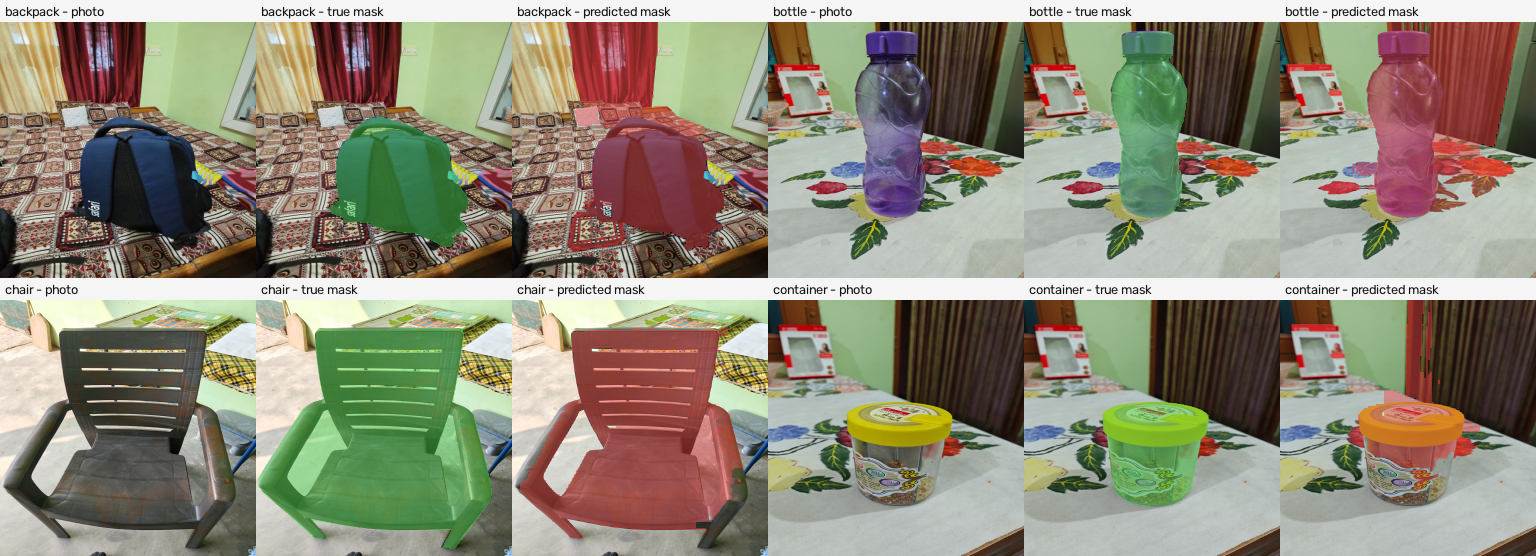
\includegraphics[width=\textwidth]{captured_grid1.png}
\caption{Captured photos 1--4. Each triple is input, true mask (green), predicted mask
(red), as semi-transparent overlays.}
\end{figure}
\begin{figure}[H]\centering
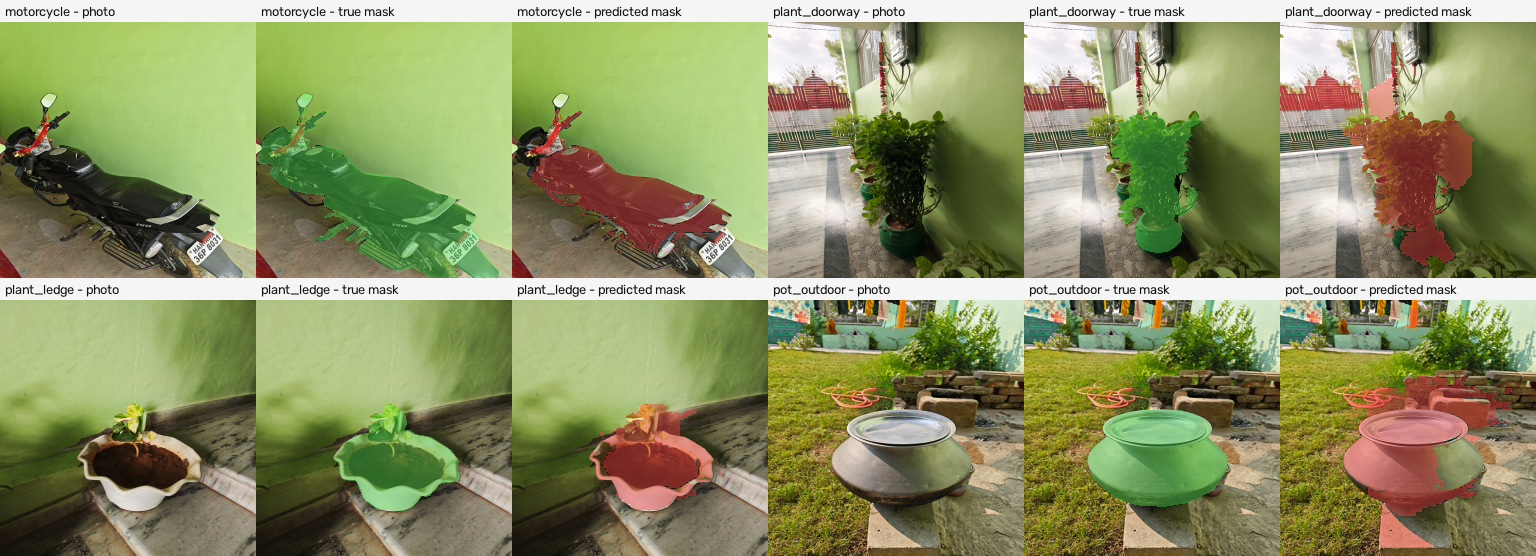
\includegraphics[width=\textwidth]{captured_grid2.png}
\caption{Captured photos 5--8, same layout.}
\end{figure}}{\emph{[Captured-photo overlays appear once the hand-drawn masks exist;
run \texttt{./finalize.sh}.]}}

\section{Failure cases}
\label{sec:failures}
\begin{figure}[H]\centering
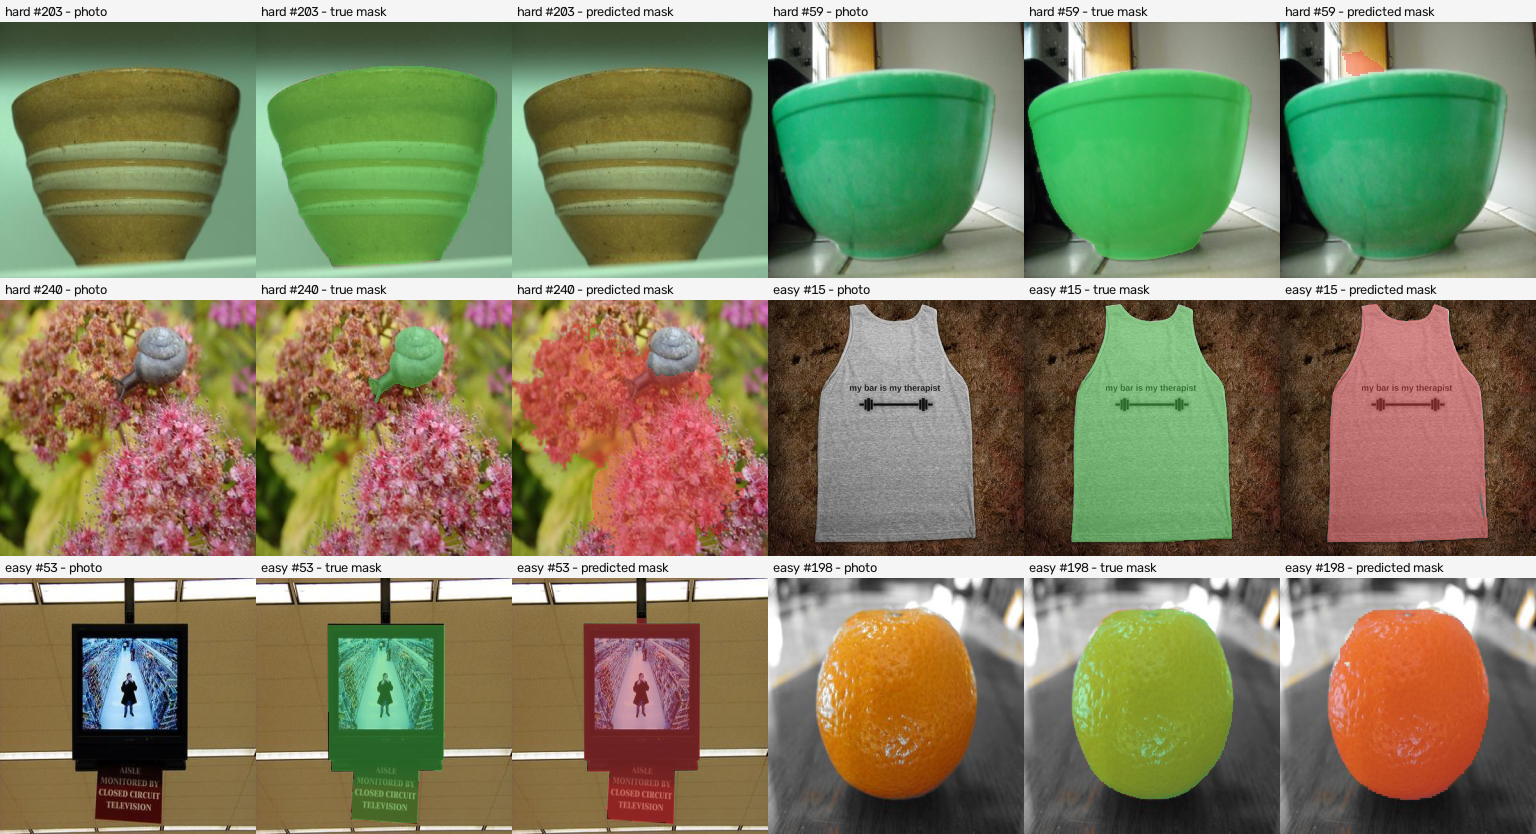
\includegraphics[width=\textwidth]{duts_examples.png}
\caption{Validation extremes: the three worst cases by IoU (first row and left of the
second), then the three best.}
\end{figure}

\textbf{1. Small or distant objects are lost entirely.} When the object covers only a
few percent of the frame it spans few regions, each carrying little unary weight because
the terminal capacities scale with pixel count $|p|$. The pairwise term, which scales
with shared border length, then overwhelms them and the cut absorbs the object into the
background. This is the dominant failure on DUTS-TE and directly explains the object-IoU
collapse in Section~\ref{sec:gap}: $22\%$ of DUTS-TE photos are in this regime versus
under $5\%$ of validation photos.

\textbf{2. Low contrast against a patterned surface.} \texttt{container} is the worst
captured photo by boundary accuracy (BF1 $0.185$ against a set mean of $\capBF$). A
translucent tub sits on a densely floral tablecloth: the colour likelihood and every
contrast cue see cloth patches that differ from their surroundings as much as the tub
does, so $P_p$ is high for both and the prediction spreads outward across the cloth.
\texttt{bottle} fails similarly (mIoU $0.606$, lowest of the eight): the bottle is
translucent, so the tablecloth shows through and the region colours inside the object
match the background.

\textbf{3. Objects merging with a similarly coloured support.} In
\texttt{pot\_outdoor} (BF1 $0.263$) a grey metal pot rests on a grey stone slab in
shadow. Region mean colours either side of the true boundary are nearly identical, so
$W_{pq}\approx1$ there and the pairwise term makes cutting between them expensive. The
smoothness prior behaves as designed; the difficulty is that the strongest edge in the
image is a brightness step inside the pot rather than at its outline. The mask absorbs part
of the slab.

\textbf{4. Thin and fragmented structure.} \texttt{plant\_doorway} (BF1 $0.328$) is
foliage with sky and wall showing between the leaves. At $\workRes^2$ the gaps are
smaller than one region, so no clustering at this resolution can represent them; the
prediction becomes a ragged blob. This is a granularity failure rather than a model
failure --- the one failure mode the oracle study in Section~\ref{sec:budget} says more
resolution would genuinely fix.

\textbf{5. Objects touching the image border.} Border contact is one of the strongest
background cues, so an object running off the frame has its border-touching regions
actively pushed towards background and the mask is clipped along the edge.

\textbf{6. Boundary quality is the weaker half of $Q$ throughout.} BF1 ($\teBF$) trails
mIoU ($\teMIoU$) on every set. Region boundaries are quantised to the $\workRes^2$ grid,
giving a $256/\workRes=2$\,px step --- right at the $5\times5$ ($\pm2$\,px) matching
tolerance, so a region edge that is slightly misplaced falls outside it. The oracle study
shows the headroom is real: a perfect region labelling at this resolution scores BF1
$0.80$, so most of the loss is the region model misplacing boundaries, not the grid.
Note the spread across the captured set is wide --- \texttt{chair} ($0.635$) and
\texttt{plant\_ledge} ($0.629$) are large, well-separated objects against plain
backgrounds, roughly double the BF1 of the cluttered cases.

\section{Reproducing}
\begin{verbatim}
python src/build_cache.py     # resize DUTS into a 256x256 cache
python src/train.py           # stats, features, logreg, tune lambda/sigma
python src/retune.py          # widen the lambda/sigma grid
python src/evaluate.py        # val + DUTS-TE + captured, and timing
python src/figures.py         # report figures
python predict.py --image photo.jpg --out mask.png
\end{verbatim}

\noindent\texttt{predict.py} prints exactly the two required lines,
\texttt{T\_CPU\_ms:} and \texttt{S\_disk\_bytes:}. It times 20 runs on the single
photo given to it, so its reported time varies with that photo's content (images with
larger objects produce more regions and a longer cut); the $\Tcpu$\,ms figure above is
the mean over all $\Ntimed$ DUTS-TE photos, which is what the CES definition uses.

\end{document}
